\documentclass[12pt,a4paper]{scrartcl}
\usepackage{forest}
\usepackage{booktabs}
\usepackage{hyperref}
\usepackage{placeins}
\usepackage{titling}
\usepackage{graphicx}
\graphicspath{{figures/}{../figures/}}
\renewcommand{\subtitle}[1]{%
  \posttitle{%
    \par\end{center}
    \begin{center}\large#1\end{center}
    \vskip0.5em}%
}
\title{Laminar fMRI pipeline}
\author{Tommy Clausner}
\subtitle{\textsc{Documentation}}
\date{\small{last updated on \today}}

\begin{document}
\begin{titlepage}
\clearpage\maketitle
\thispagestyle{empty}
\end{titlepage}
\tableofcontents
\newpage
\listoffigures
\newpage
\listoftables
\newpage
\section{Pre- requisites}
\begin{itemize}
\item MRIcron (\href{https://www.nitrc.org/projects/mricron}{https://www.nitrc.org/projects/mricron})
\item FSL (\href{https://fsl.fmrib.ox.ac.uk/fsl/fslwiki}{https://fsl.fmrib.ox.ac.uk/fsl/fslwiki})
\item FreeSurfer (\href{https://surfer.nmr.mgh.harvard.edu/}{https://surfer.nmr.mgh.harvard.edu/})
\item SPM (\href{http://www.fil.ion.ucl.ac.uk/spm/}{http://www.fil.ion.ucl.ac.uk/spm/})
\item analysePRF (\href{http://kendrickkay.net/analyzePRF/}{http://kendrickkay.net/analyzePRF/})
\item knkutils (\href {https://github.com/kendrickkay/knkutils/}{https://github.com/kendrickkay/knkutils/})
\item Open fMRI Analysis (\href{https://github.com/TimVanMourik/OpenFmriAnalysis}{https://github.com/TimVanMourik/OpenFmriAnalysis})
\item MATLAB R2015a or later (\href{https://nl.mathworks.com/products/matlab.html}{https://nl.mathworks.com/products/matlab.html})
\item Tommy's Scriptinator 3000 TM (optional; \href{https://github.com/TommyClausner/Scriptinator}{https://github.com/TommyClausner/Scriptinator})
\end{itemize}

Use e.g. MRIcron's dicom2nii to convert raw MRI data to NifTi files.\\

\section{Folder structure}
The general folder structure is set up by a call to setupfolders.sh (see also Figure \ref{tree:folderstruct})
\begin{itemize}
\item Functional data must be located in niftis/\textbf{functionals}/
\item Anatomical data must be located in niftis/\textbf{t1}/
\item Inverted functional data must be located in niftis/\textbf{inverted}/
\item Proton density data must be located in niftis/\textbf{pd}/
\item Inverted proton density data must be located in niftis/\textbf{pdinverted}/
\end{itemize}

\section{How things work}
Parts of the analysis run in Bash shell scripts. Those can be called from their root directory using "sh scriptname.sh" (excl. quotation marks). Each step within the analysis has a different subfolder containing the respective results of this step. Leading numbers indicate in which logical order the corresponding shell scripts should be executed. Note that all files created by each respective step are stored in the coresponding folder. However files that need to be preset (e.g. config files) must be located in A\_helperfiles. Note Further, that the entire analysis can be broken down to a few sub-pipelines. Those are explained in a individual section.\\

\noindent All functions with the prefix \textit{do\_} will affect the data.

\section{Suggested order of operations}
\begin{itemize}
\item makenewsubject.sh
\item copy NifTi files to the correct location (see above)
\item open terminal (the following are terminal commands)
\item cd PATH/SUBJECTFOLDER/B\_scripts
\item sh runonqsub.sh 32gb do\_preparefunctionals.sh
\end{itemize}
\subsection{Pre-processing}
\begin{itemize}
\item sh runonqsub.sh 32gb do\_realignment.sh
\item sh runonqsub.sh 32gb do\_distcorr.sh
\item sh runonqsub.sh 64gb do\_applysimpledistcorr.sh
\item sh runonqsub.sh 16gb do\_preparecoregistration.sh
\item sh do\_correctavgdiff.sh
\end{itemize}
\subsection{Co-registration and masks}
\begin{itemize}
\item sh runonqsub.sh 16gb do\_fsrecon.sh
\item sh do\_coregistration.sh
\item sh runonqsub.sh 16gb do\_makemasksandlabels.sh
\end{itemize}

\begin{figure}[h]
\begin{center}
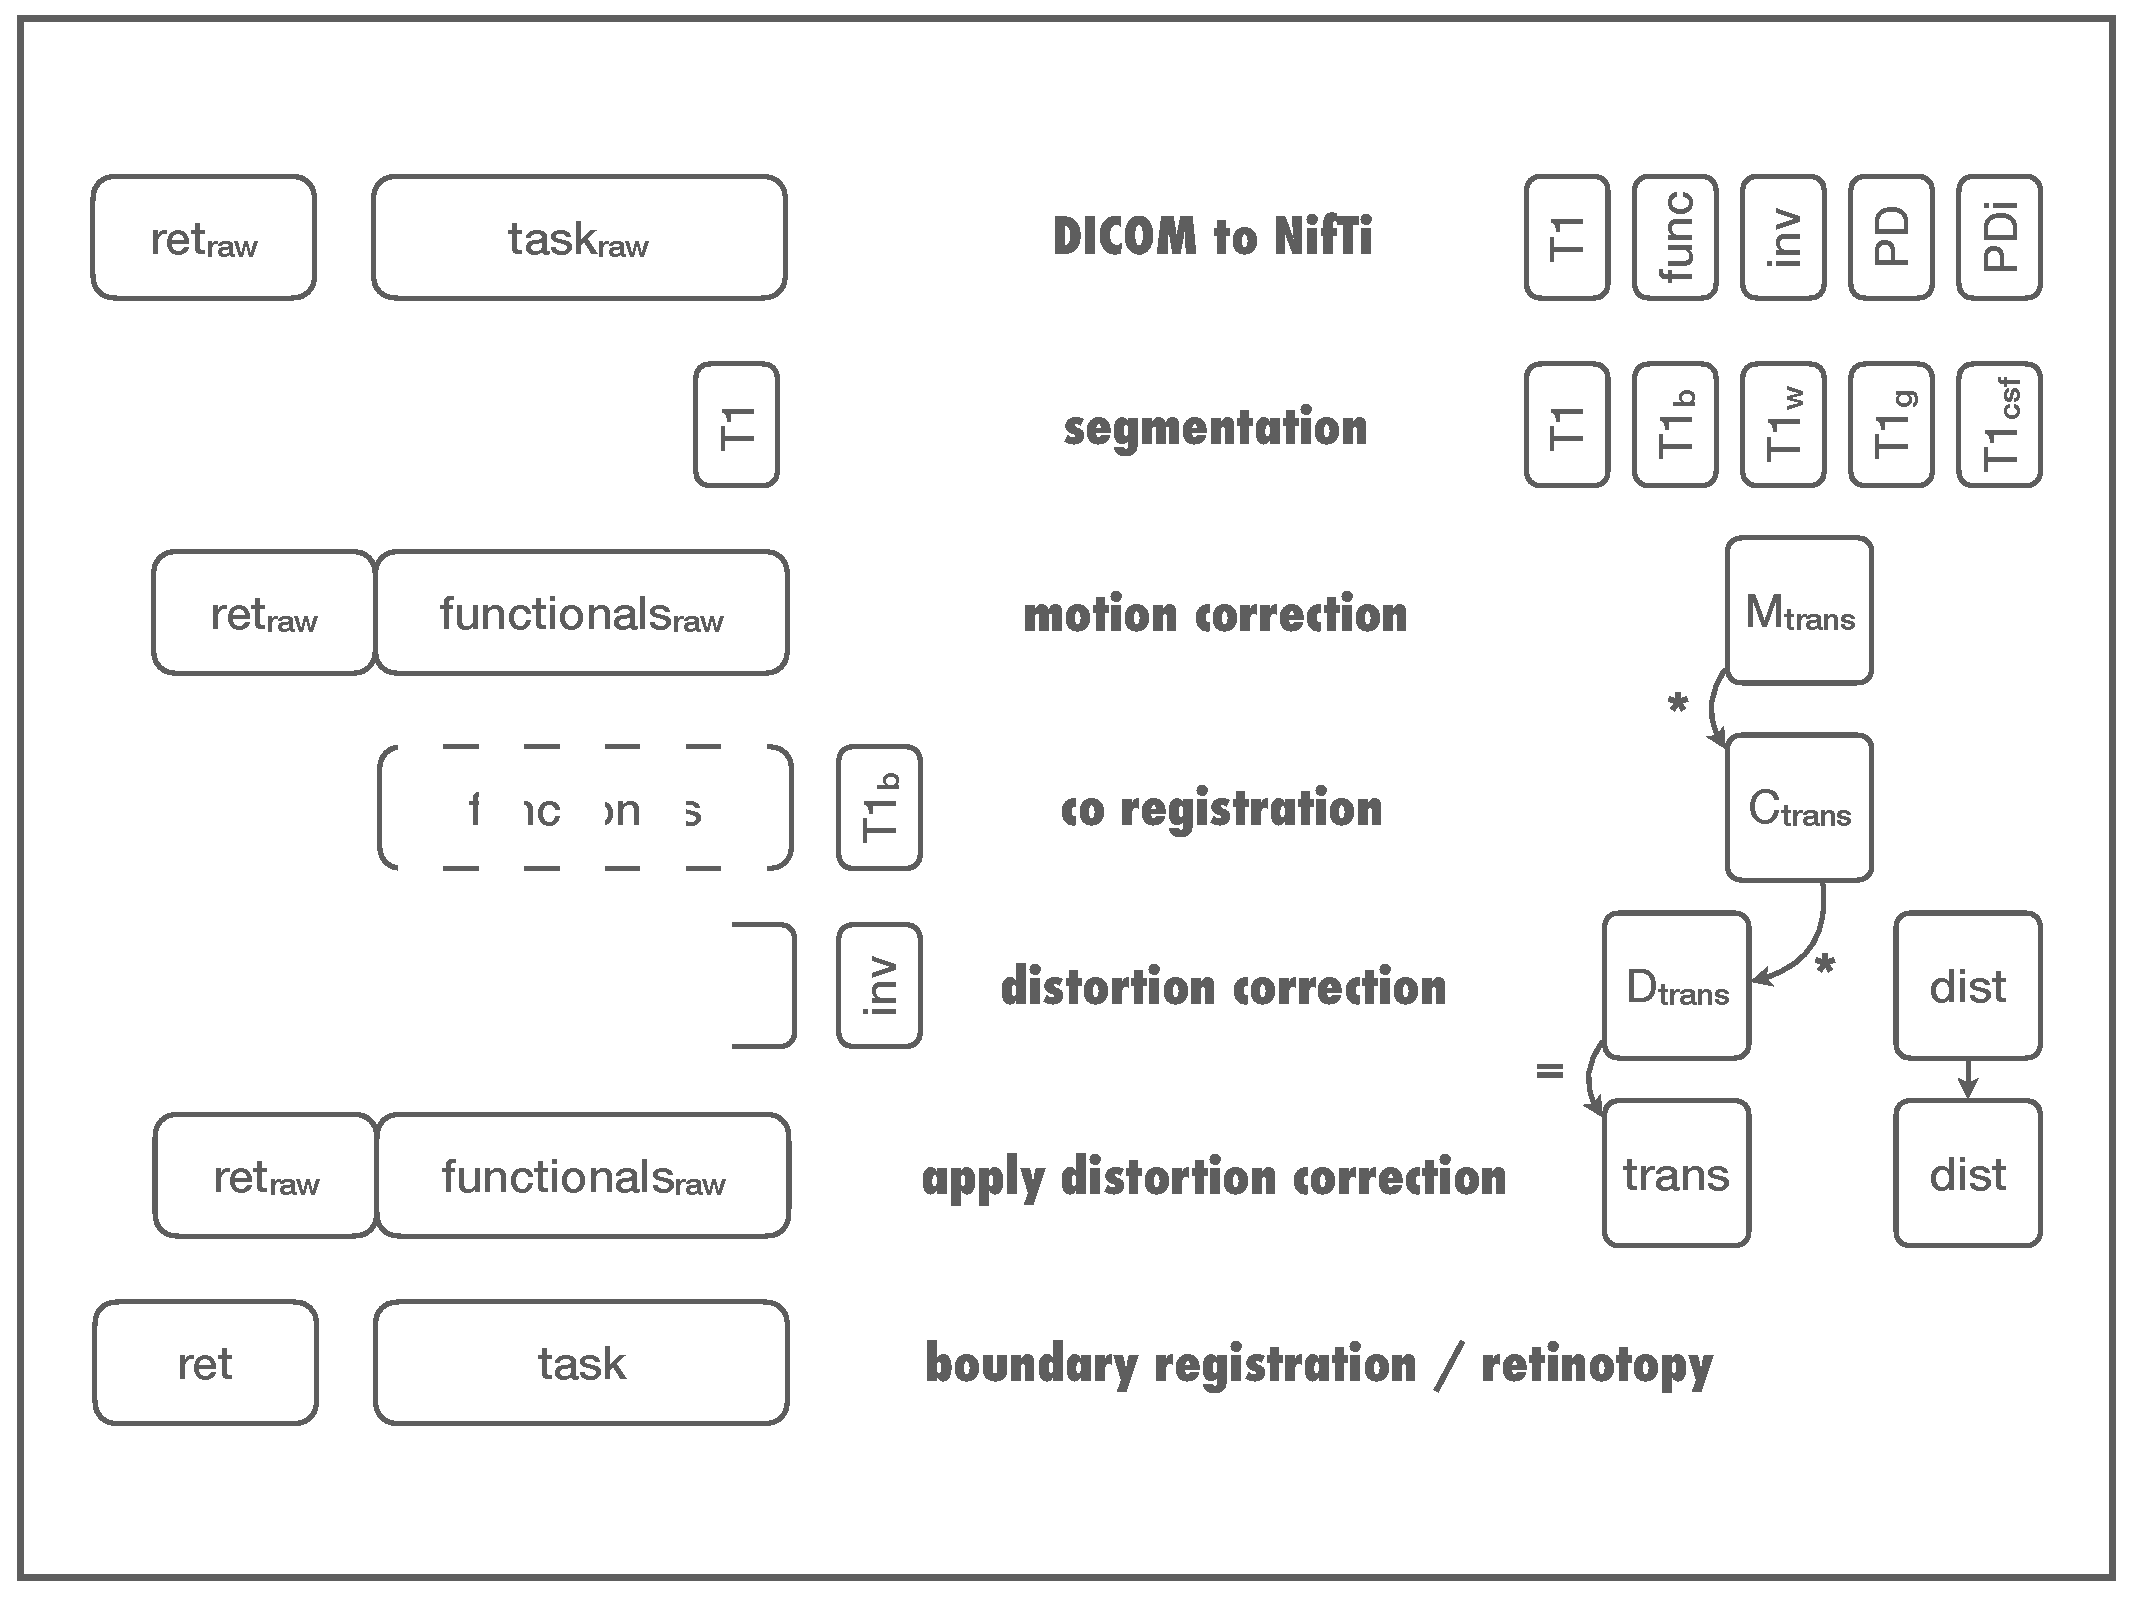
\includegraphics[width=0.8\textwidth]{overviewpreprocmain}
\caption[Overview Pre-processing fMRI]{Overview Pre-processing fMRI}
\end{center}
\end{figure}
\begin{figure}[h]
\begin{center}
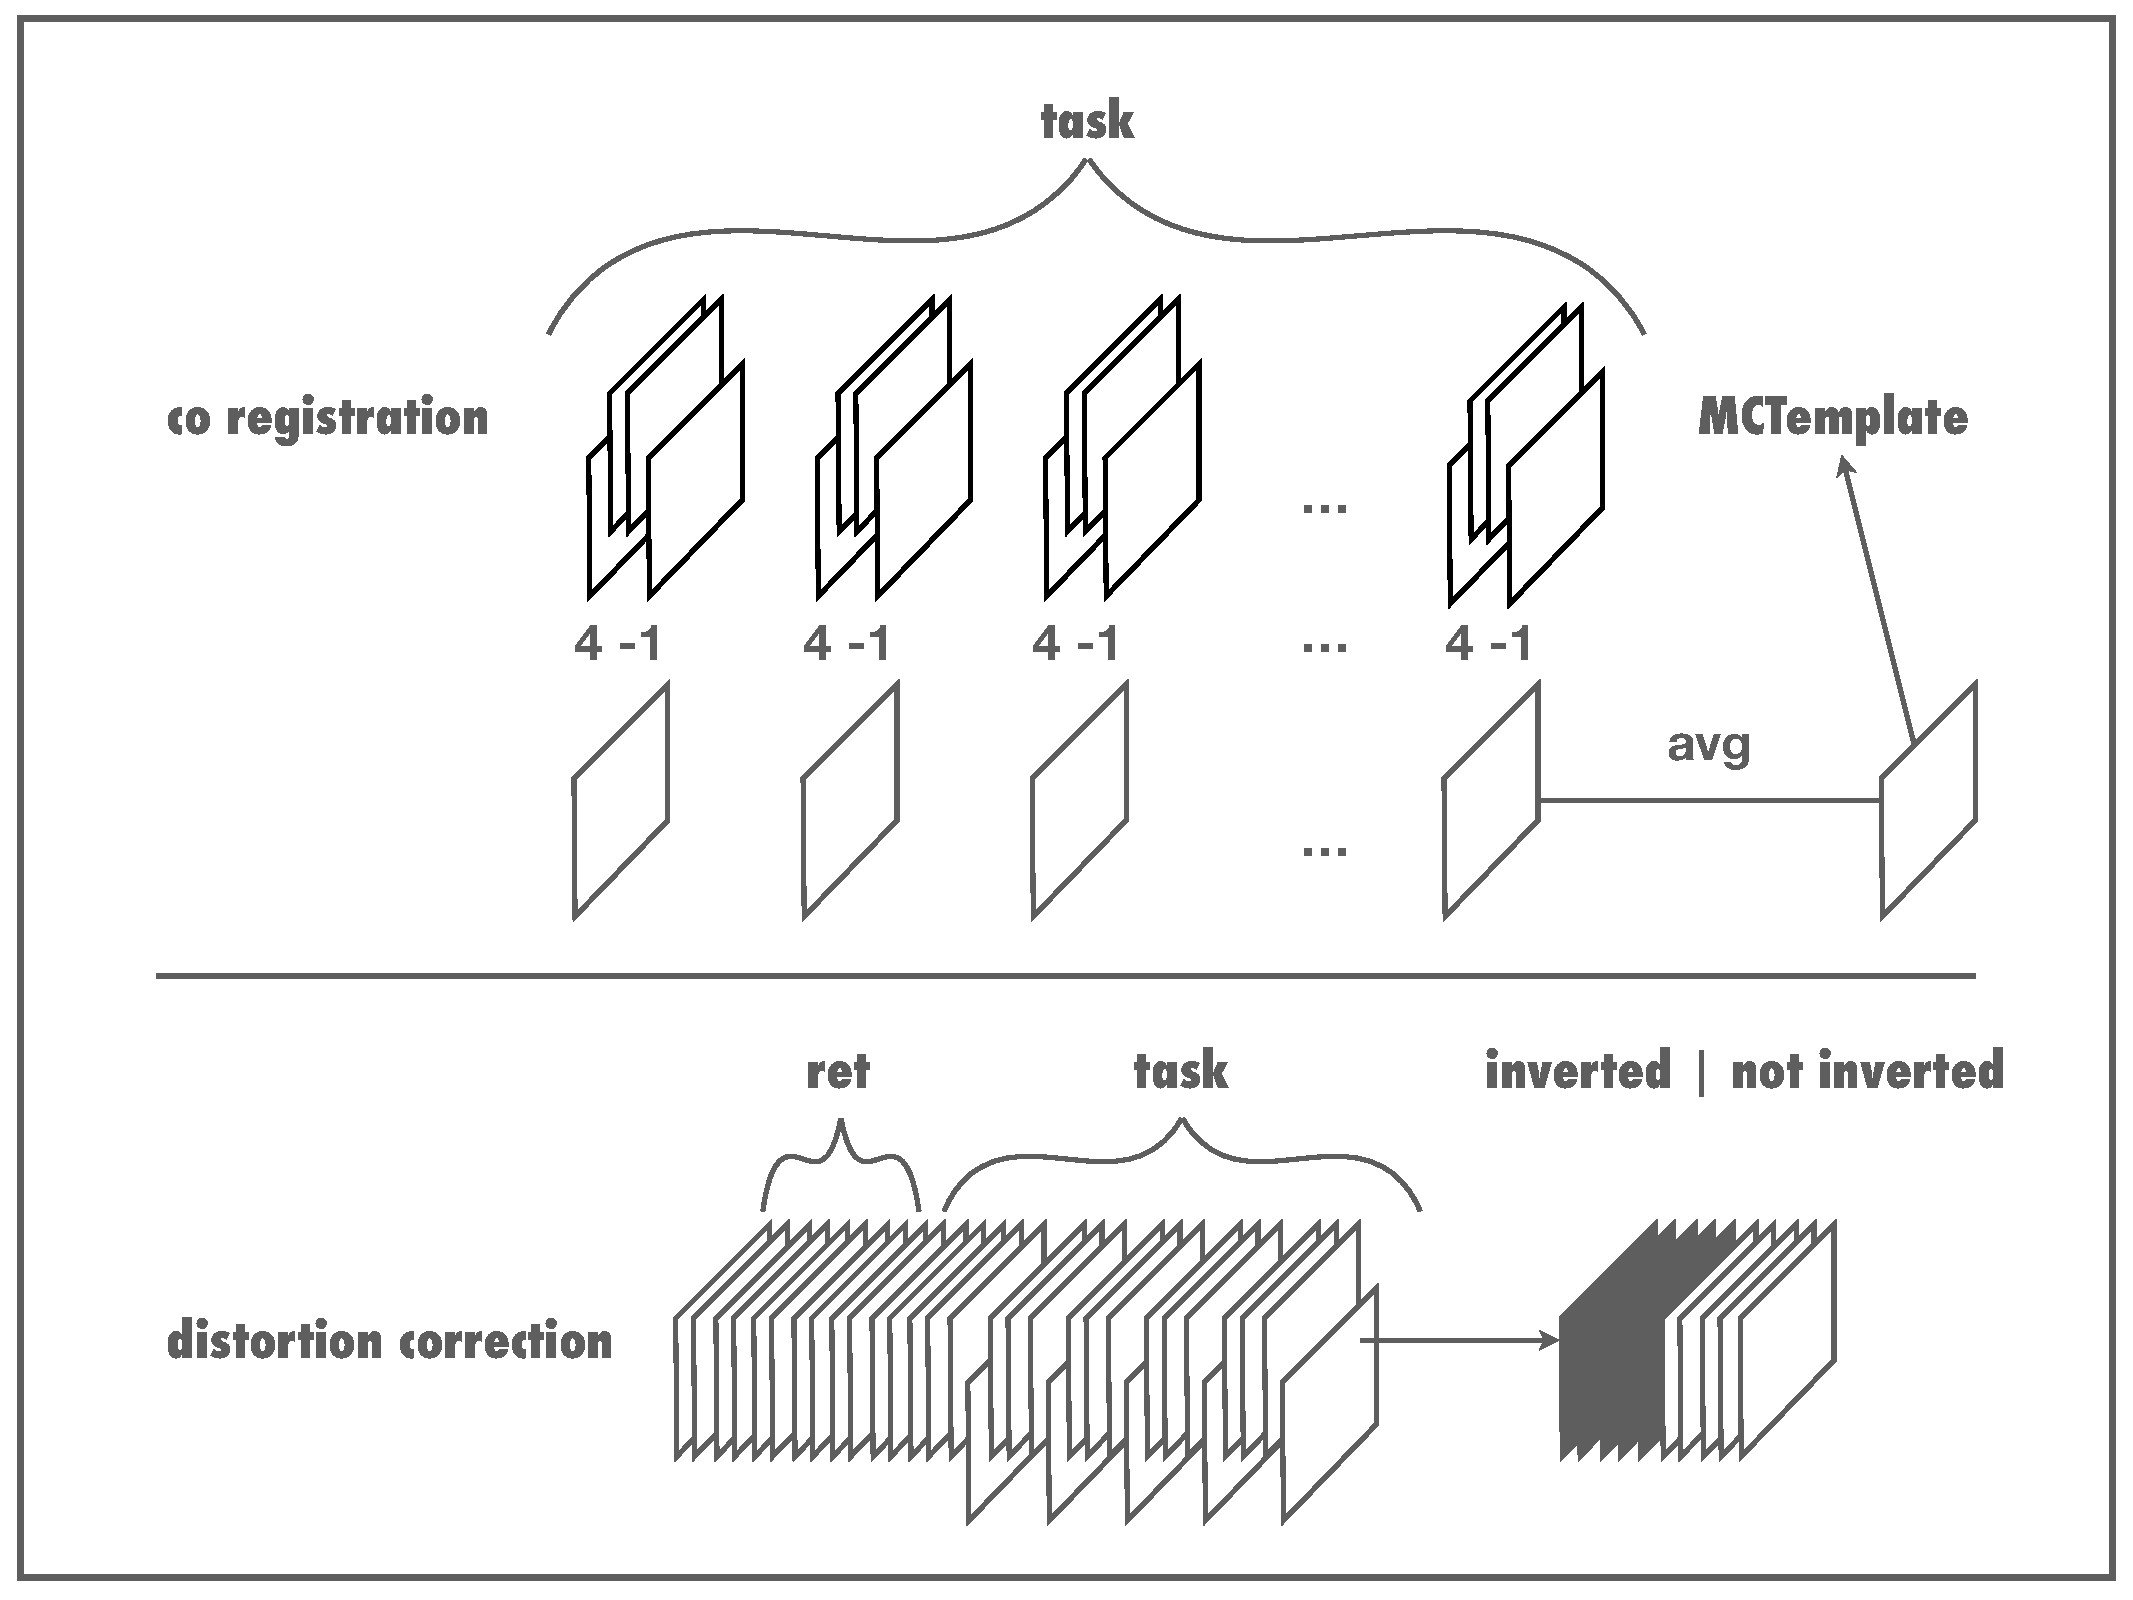
\includegraphics[width=0.8\textwidth]{coregdist}
\caption[Coregistration and distortion correction visual depiction]{Coregistration and distortion correction visual depiction}
\end{center}
\end{figure}
\begin{figure}[h]
\begin{center}
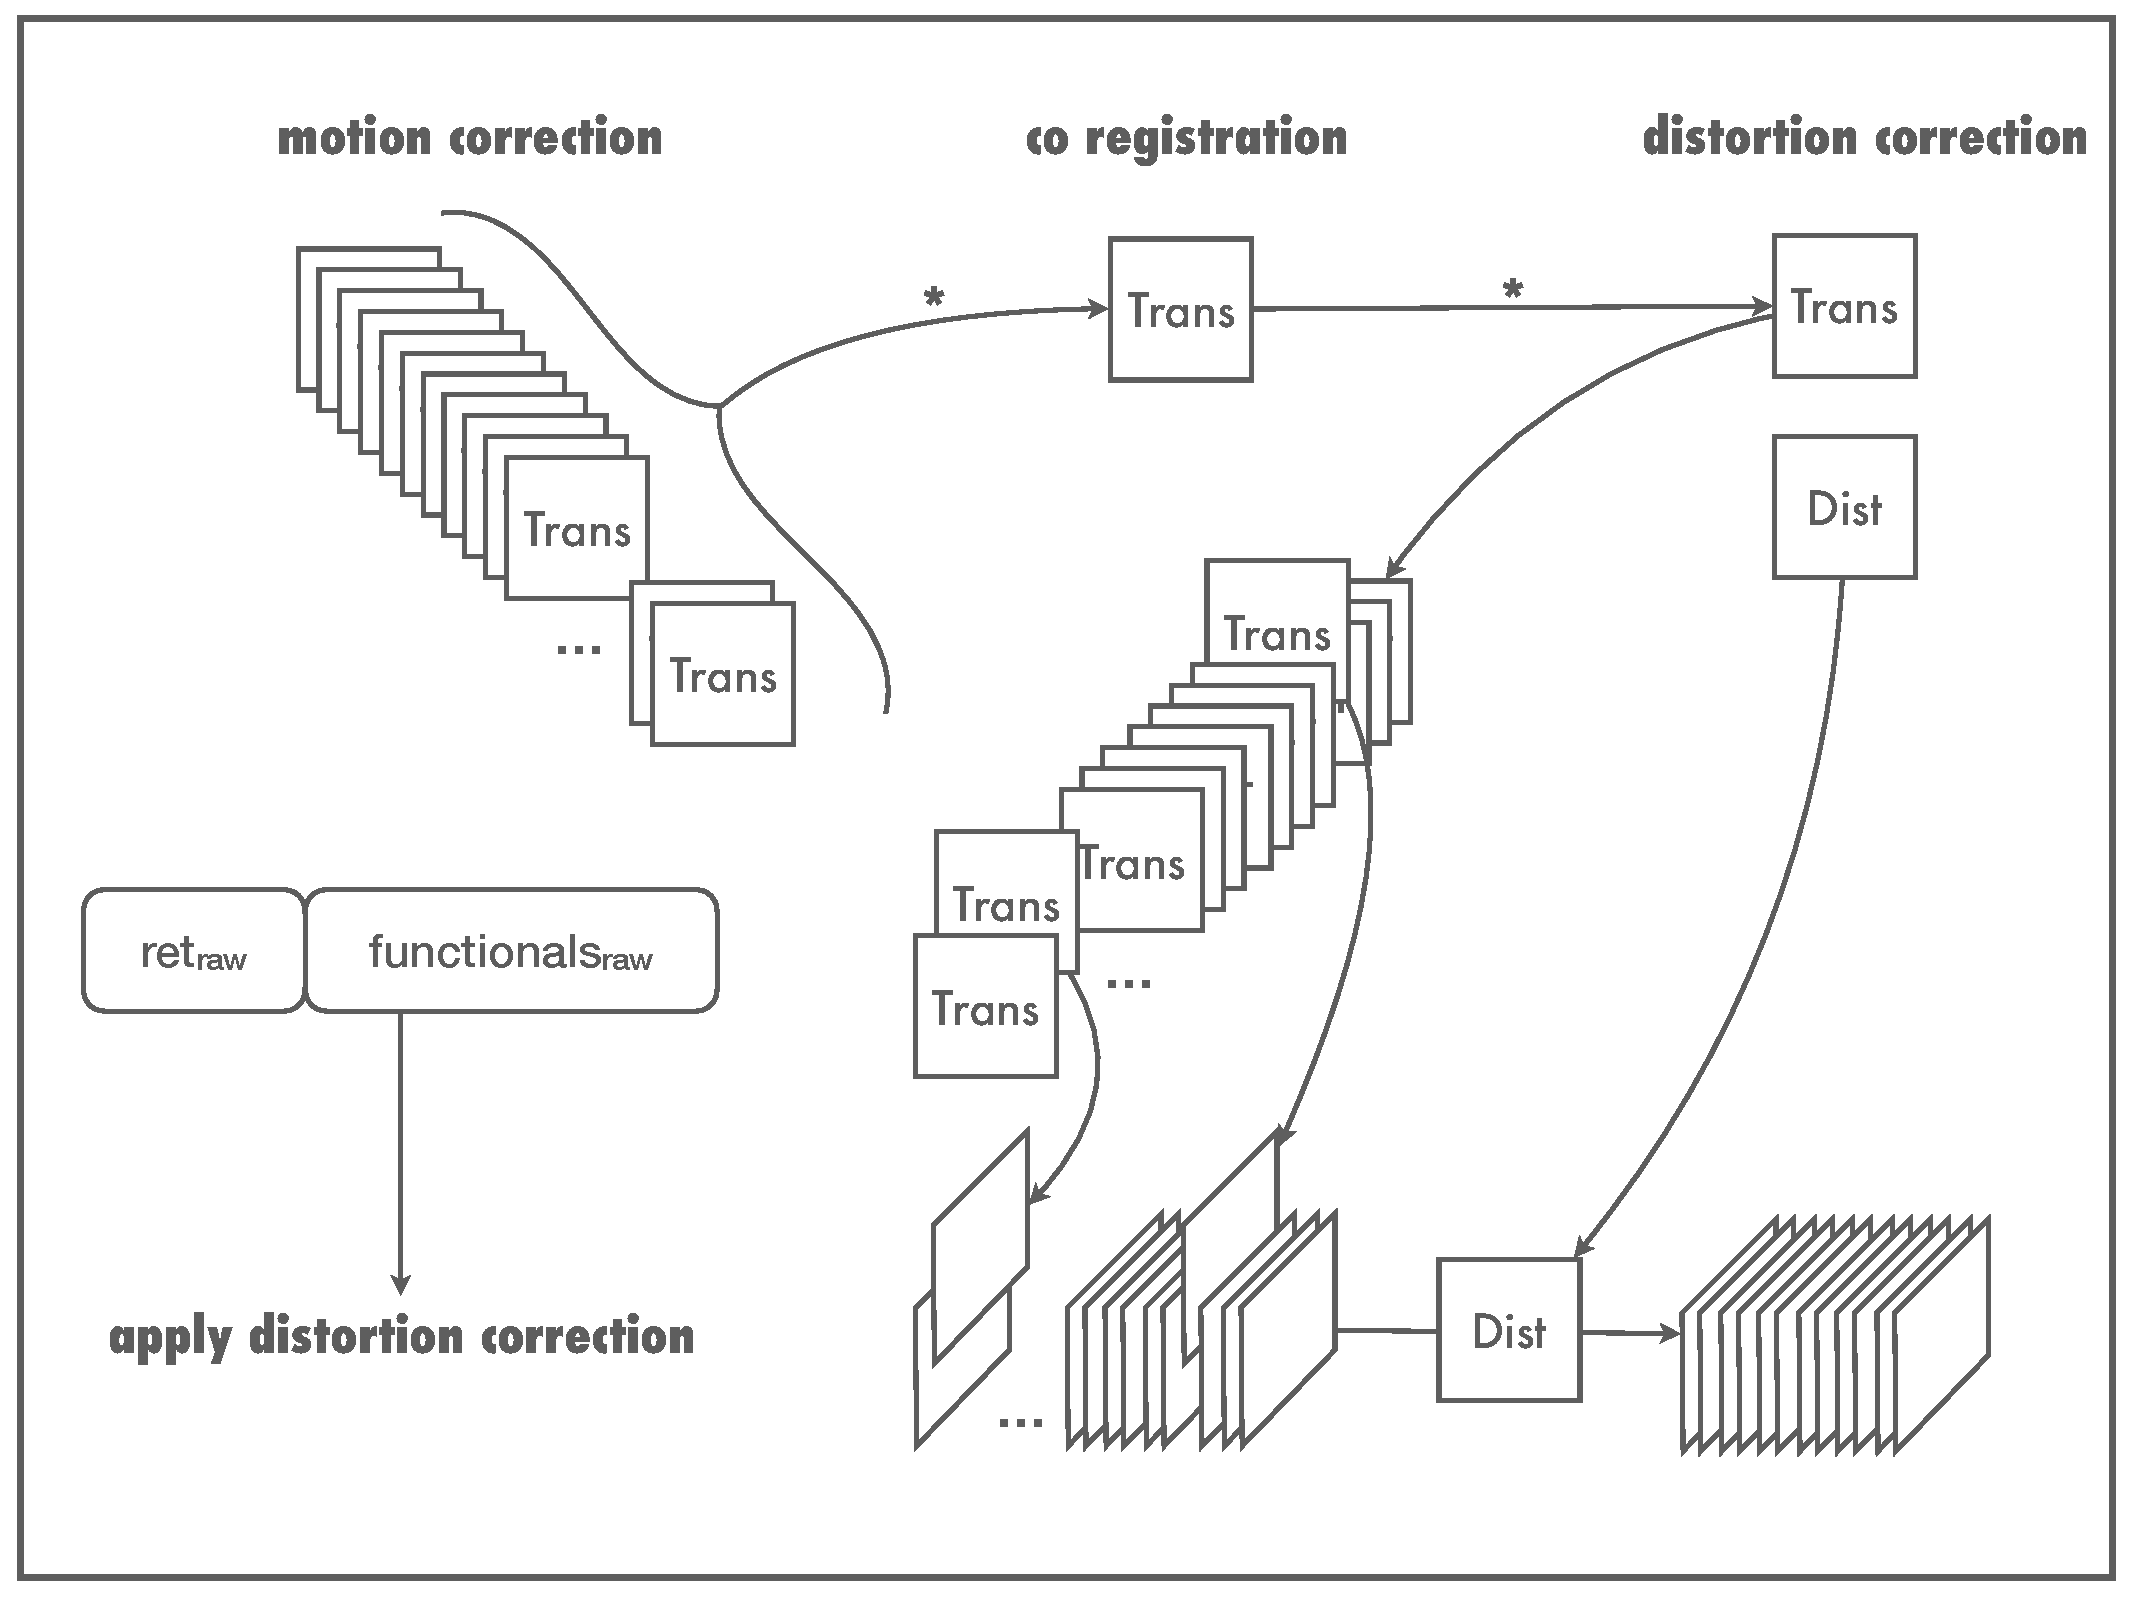
\includegraphics[width=0.8\textwidth]{applycorr}
\caption[Apply corrections from all steps at once]{Apply corrections from all steps at once}
\end{center}
\end{figure}

\FloatBarrier
\subsection{Retinotopy}
\begin{itemize}
\item sh do\_tseriesinterpolation.sh
\item sh do\_split\_analyzePRF.sh
\item sh combine\_split\_PRF\_results.sh
\item sh make\_PRF\_overlays.sh
\item sh runonqsub.sh 16gb makeOverlays.sh
\end{itemize}
\subsection{laminar separation}
\begin{itemize}
\item sh GUI2ROIs.sh
\item sh labels2masks.sh
\item sh expandROIs.sh
\item sh do\_getLayers.sh
\item sh do\_getLayerWeights.sh
\end{itemize}
\section{qsub}
Scripts that are flagged with the (Q) can be run as a qsub job.

\noindent When running the computation on the cluster use the wrapper function runonqsub.sh\\

\noindent Note that some scripts send a MATLAB script to the qsub cluster. Thus they cannot be run using runonqsub.sh, but instead create their own job.\\

\noindent Some scripts are present as scriptnameQsub.sh Those scripts contain an internal Qsub-wrapper and do the same as sh runonqsub.sh XXgb scriptname.sh\\

\noindent the following requirements on memory and computation time can be expected:

\begin{table}[h]
\centering
\begin{tabular}{l | r | l}
\toprule
script & memory required & time required\\\hline
	do\_preparefunctionals.sh & 32GB & $\approx 10min$ \\\hline
  do\_realignment.sh & 32GB & $\approx 30min$ \\\hline
  do\_distcorr.sh & 32GB & $\approx 15min$ \\\hline
  do\_applysimpledistcorr.sh & 32GB & $\approx 30min$ \\\hline
  do\_preparecoregistration.sh & 16GB & $\approx 4.5h$ \\\hline
  do\_correctavgdiff.sh & 4GB & $\approx 3sec$ \\\hline
	do\_fsrecon.sh & 16GB & $\approx 6h$ \\\hline
  do\_coregistration.sh & 16GB & $\approx 30min$ \\\hline
	do\_makemasksandlabels.sh & 16GB & $\approx 1min$ \\\hline
	do\_tseriesinterpolation.sh & 64GB & $\approx 20min$ \\\hline
	do\_split\_analyzePRF.sh & 480GB & $\approx 7h$ \\\hline
	combine\_split\_PRF\_results.sh & 64GB & $\approx 10min$ \\\hline
  make\_PRF\_overlays.sh & 16GB & $\approx 10min$ \\\hline
	makeOverlays.sh & 16GB & $\approx 5min$\\\hline
	GUI2ROIs.sh & 8GB & user dependent \\\hline
  labels2masks.sh & 8GB & $\approx 10s$ \\\hline
  expandROIs.sh & 16GB & $\approx 3min$ \\\hline
  do\_getLayers.sh & 16GB & $\approx 20min$ \\\hline
  do\_getLayerWeights.sh & 16GB & $\approx 5min$ \\\bottomrule
\end{tabular}
\caption[Approximated time and memory requirements when running on qsub]{Approximated time and memory requirements for the respective script to run. Note that everything that is more than 4GB should be run on the cluster. Use runonqsub.sh for that purpose.}
\label{tab:hardwarerequirements}
\end{table}

\newpage
\begin{figure}
\caption{Initial folder structure as required for the analysis}
\vspace{10pt}
{\footnotesize
\begin{forest}
  for tree={
    font=\ttfamily,
    grow'=0,
    child anchor=west,
    text height=0.05cm,
    parent anchor=south,
    anchor=west,
    calign=first,
    edge path={
      \noexpand\path [draw, \forestoption{edge}]
      (!u.south west) +(12pt,0pt) |- node[fill,inner sep=1.25pt] {} (.child anchor)\forestoption{edge label};
    },
    before typesetting nodes={
      if n=1
        {insert before={[,phantom]}}
        {}
    },
    fit=band,
    before computing xy={l=20pt},
  }
  [Analysis folder
[toolboxes/
    [analyzePRF-1.1/]
    [knkutils-master/]
    [OpenFmriAnalysis-master/]
    [spm12/]
  ]
[S\#/ (set up by setupfolders.sh or when created using makenewsubject.sh)
  [0\_freesurfer/
  ]
  [1\_realignment/
  ]
  [2\_coregistration/
  ]
  [3\_distcorrection/
  ]
  [4\_retinotopy/
  ]
  [5\_laminar/
  ]
  [A\_helperfiles/
    [acquisition\_parameters.txt]
    [b02b0.cnf]
    [b02b0\_example\_fsl.cnf]
    [params.mat]
    [images.mat]
  ]
  [B\_scripts/
    [*.m]
    [*.pipe]
    [*.sh]
  ]
  [C\_miscResults/
  ]
  [niftis/
  [functionals/]
  [inverted/]
  [pd/]
  [pdinverted/]
  [t1/]
  ]
]
[template\_session/
[template\_helperfiles/
	[acquisition\_parameters.txt]
  [b02b0.cnf]
  [b02b0\_example\_fsl.cnf]
  [params.mat]
  [images.mat]
]
[template\_scripts/
	[*.m]
  [*.pipe]
  [*.sh]
]
]
[makenewsubject.sh]
]
\end{forest}

}
\label{tree:folderstruct}
\end{figure}

\FloatBarrier
\section{Helper files}
There are several helper files that are needed in order to perform the analysis:

\subsection{acquisition\_parameters.txt}
indicating the respective acquisition parameters per volume needed in order to perform the distortion correction. One line indicates the respective parameter setting for the respective volume (1st line corresponds to 1st volume, etc.)\\

\noindent e.g.:

\noindent 0 1 0 0.042\\
\noindent 0 -1 0 0.042\\

The first 3 columns indicate the respective phase coding direction the last column some weird value, that is only important if it changes. Otherwise it's fine to use any value as long as it is the same.

\subsection{b02b0.cnf}
Settings for distortion correction.

Needed in order to set the parameters for the distortion correction (example provided by FSL).

\subsection{params.mat}
Parameters used for retinotopy scans as obtained from VistaDisp.

\subsection{images.mat}
Stimuli used for retinotopy scans. Stimuli file must be such that each frame is represented as a binary image. The matrix must be of shape $Y \times X \times T$ where $X$ and $Y$ are the image dimensions in pixel and T is the respective number of frames.

\section{Scripts explained (support for runonqsub.sh: Q)}
\subsection{runonqsub.sh}
Initiates a qsub session and sends it to the cluster. This is necessary, since scripts running on the cluster are copied to a different directory, but within scripts all directories are relative. runonqsub.sh must hence be run in a "normal" session not using a non-interactive qsub, giving the respective script that was intended to run as an argument. runonqsub will then set everything up correctly. Further you have to specify the amount of memory needed.\\

example: sh runonqsub.sh 32gb myscript.sh\\

\noindent Additional arguments can be passed after the script.\\

example: sh runonqsub.sh 32gb myscript.sh myargument\\

\noindent Under the hood:
\begin{itemize}
\item a qsub session is initiated like so: qsub -l walltime=24:00:00,mem=\$1 -F "\$DIR \$\{@:3\}" \$DIR/\$2
\item \$DIR is the current absolute path to B\_scripts
\item \$1 is the amount of memory used (e.g. 32gb)
\item \$2 is the respective script to run (e.g. myscript.sh)
\item \$\{@:3\} is all following arguments that are parsed to the script
\item every time runonqsub.sh is called the absolute path is forwarded to the script (-F \$DIR) in order to keep the relative dependencies clear
\end{itemize}

\subsection{cleanscriptsfolder.sh}
Since qsub puts a output + error log into /B\_ scripts cleanscriptsfolder.sh can be used to move all qsub outputs to /B\_scripts/qsuboutput\\

\subsection{liveupdateqsub.sh}
Submits a qstat -u user request every second.\\

example: sh liveupdateqsub.sh tomcla\\

\noindent exit command by hitting ctrl+c

\subsection{waitForJobs.sh}
Checks all currently running jobs (qstat -u user) and waits until the last script up until this point has finished.

\subsection{makenewsubject.sh}
executable script (double click to execute)\\

Creates a new subject (S\#) folder structure in order to get all folder dependencies right. It automatically detects folders called "S\textit{number}" and creates a new folder incrementing \textit{number} by one

\subsection{setupfolders.sh (Q)}
Sets up the necessary folder structure for the analysis (within a subject folder). This function is automatically called when using makenewsubject.sh\\

\noindent example: sh setupfolders.sh

\subsection{do\_preparefunctionals.sh (Q)}
Prepares functional data, i.e. removes the first 4 and the last x volumes of every set of functionals, where x is the number of volumes acquired after the stimulation ended. If files were modified (i.e. if volumes were deleted), the original file will remain in /niftis/functionals/old\\

\noindent example: sh do\_preparefunctionals.sh\\

\subsection{do\_realignment.sh (Q)}
example: sh do\_realignment.sh\\

\noindent Merges and motion corrects all files in /niftis/functionals using the average volume of all task volumes.\\

\noindent numberofvolumes.txt is written to /A\_helperfiles giving information about which sets had how many volumes. The first column is coresponds to dim4 from fslinfo\\

\noindent Under the hood:
\begin{itemize}
\item fslmerge is called to create a combined .nii for all files in niftis/functionals/*sparse* - files are merged allong the 4th dimension
\item a .txt file is created saving which files were merged and how many volumes were in there
\item mcflirt is used on the combined data doing the motion correction based on the average volume across all task blocks
\item all results are stored in /1\_realignment
\item results have the extension "\_mcf"
\end{itemize}

\subsection{do\_distcorr.sh (Q)}
example: sh do\_distcorr.sh\\

\noindent Uses the averge volume of the inverted set of images in /niftis/inverted as reference for \textit{inverted}\\

\noindent Uses as many volumes \textit{n} as there were in /niftis/inverted. Respective volumes are selected starting from the last going in \textit{4 x n} steps backward. Hence the resulting average of this set was computed over the 4th volume of each of \textit{n} last sets in the normal images. Simplified (all 1 are selected):\\

\noindent for n=5\\

\noindent 0,0,0,0,...,0,0,0,1,0,0,0,1,0,0,0,1,0,0,0,1,0,0,0,1\\

\noindent Both (normalavg and invertedavg) will be used to esimate the distortion correction.\\

\noindent Under the hood:
\begin{itemize}
\item reference volumes (normal + inverted) are selected in order to do the field distortion estimate (selection: see above).
\item selected reference volumes are merged into a single file (/3\_distcorrection/all\_b0.nii.gz)
\item topup is called using the merged (normal + inverted) .nii and performs field mapping accoriding to the specifications in /A\_helperfiles/b02b0.cnf using the acquisition parameters specified in acquisition\_parameters.txt
\item all results are stored in /3\_distcorrection
\end{itemize}

\subsection{do\_applysimpledistcorr.sh (Q)}
Applies distortion correction to all functional data.\\

\noindent example: sh do\_applydistcorr.sh\\

\noindent Under the hood:
\begin{itemize}
\item distortion correction is applied to the full set of functionals using the OUTPUT of topup (topup [$\ldots$] --out=OUTPUT) as well as acquisition\_parameters.txt (Using --method=jac)
\item all results are stored in /3\_distcorrection
\item all results have the prefix "corrected\_"
\end{itemize}

\subsection{do\_preparecoregistration.sh (Q)}
Computes a reference volume (MCTemplate) used as the basis  to co-register with the anatomical image. This image is computed by splitting the entire set of task volumes into chunks of 4. In each chunk the 1st volume is substracted from the 4th. This procedure yields a pseude-T1 contrast. All chunk differences are then averaged to form "MCTemplate"

\noindent example: sh do\_preparecoregistration.sh

\subsection{do\_correctavgdiff.sh (Q)}
Due to the subtraction of the 1st from the 4th volume the area outside the brain has the highest value. In order to correct this the lowest value will be shifted to zero the a certain part of the higher values are cut (e.g. 0.975).\\

\noindent example: sh do\_correctavgdiff.sh\\

\noindent The result should be checked using "fsleyes ../2\_coregistration/Inplane/MCTemplateThr*.nii.gz" to ensure that the area outside the brain is nulled. Note that it can happen that some areas within the brain are nulled as well. If they are not too wide spread they do not affect later coregistration.

\subsection{do\_fsrecon.sh (Q)}
Performs segmentation using Freesurfer.\\

\noindent If running on OSX the script assumes:\\
\noindent FREESURFER\_HOME=/Applications/freesurfer\\

\noindent If running on linux the script assumes:\\
\noindent FREESURFER\_HOME=/opt/freesurfer/version\\

\noindent The target image that is used for the segmentation must be located in /niftis/t1\\

\noindent example: sh do\_fsrecon.sh\\

\noindent Under the hood:
\begin{itemize}
\item calls recon-all -i /niftis/t1/* -subjid  0\_freesurfer -all
\item all results are stored in /0\_freesurfer
\end{itemize}

\subsection{do\_coregistration.sh}
Will submit a qsub session using MATLAB, that in turn will be using FreeSurfer (bbregister) and OpenFmriAnalysis to perform a linear and non-linear boundary registration.  Movie files of the respective co-registration are stored in /C\_miscResults

\noindent The file used to execute MATLAB commands is /B\_scripts/do\_coregistration.m Note that it will be modified using the correct folder settings, which yields tmp.m that will be called and removed after MATLAB was closed.\\

example: do\_coregistration.sh

\subsection{do\_coregistration.m}
The script doing the actual co-registration. Uses wrapper functions from OpenFmriAnalysis to evoke FreeSurfers bbregister and computes a recursive boundary based registration.\\

\noindent The results are seevral files storing the boundaries as a point cloud, and the respective transformation in diferent formats.

\noindent Under the hood:
\begin{itemize}
\item calls bbregister
\item results are stored in /2\_coregistration
\item yields boundaries.mat, matrix.mat, bbregister.dat, transmat.txt, transmatinv.txt
\end{itemize}

\subsection{do\_makemasksandlabels.sh (Q)}
example: sh do\_makemasksandlabels.sh\\

\noindent Uses FreeSurfer reconstruction to create masks for CSF, gray matter and white matter and creates labeled volume for use within retinotopy containing left / right + gray / white matter. All masks will be created as full-brain and partial-brain masks.\\

\noindent If the orientation needs to be changed, parse the respective FreeSurfer compatible orientation parameter (\href{https://surfer.nmr.mgh.harvard.edu/pub/docs/html/mri_convert.help.xml.html}{https://surfer.nmr.mgh.harvard.edu/pub/docs/html/mri\_convert.help.xml.html})\\

\noindent example: sh do\_makemasksandlabels.sh

\noindent Under the hood:
\begin{itemize}
\item moves anatomical volumes to functional space calling do\_movesinglevolume.sh InputVolume.nii.gz transmat.txt OutputVolume.nii.gz
\item results are stored in /2\_coregistration
\item coregistered functional masks have the prefix "fct" and the suffix "coreg"
\end{itemize}

\subsection{do\_movesinglevolume.sh}
Simple wrapper function to apply a transformation from one volumetric space to another, given a transformation matrix.\\

\noindent example: sh do\_movesinglevolume.sh

\noindent Under the hood:
\begin{itemize}
\item flirt -applyxfm -in \$1 -ref \$1 -init \$2 -out \$3
\item \$1: volume to move
\item \$2: transformation matrix in form of a .txt file containing a $4\times4$ transformation matrix
\end{itemize}

\subsection{do\_tseriesinterpolation.sh}
Wrapper function for do\_tseriesinterpolation.m Variables used by do\_tseriesinterpolation.m can be defined in the header section of the script.

\noindent example: do\_tseriesinterpolation.sh

\noindent Under the hood:
\begin{itemize}
\item submits a MATLAB job using qsub calling do\_tseriesinterpolation.m using the below settings
\item default number of blocks: 3
\item default TR: 2.7s
\item default Mask Threshold: 0.01
\item default rescaled stimulus size: 100px
\end{itemize}

\subsection{do\_tseriesinterpolation.m}
Interpolates time series for retinotopy scans to match the number of frames during the stimulation (cubic interpolation). The new TR will be $TR_{new}=\frac{TR_{old}N_{volumes}}{N_{imageframes}}$. The function implements "tseriesinterp" from the analyzePRF toolboxe. The data will be normalized to percent signal change.\\

\noindent Furthermore all images will be downsampled to the predefined size (e.g. 100px)\\

\noindent Under the hood:
\begin{itemize}
\item interpolates time series of functional data to match the numer of frames during the stimulation
\item results: tIntData.mat (interpolated time series)
\item results: mask.mat (volume mask)
\item results: voxelindices.mat (indices of mask voxels, ratio between $N_{imageframes}$ and $N_{volumes}$, mask threshold)
\item results: downsampled images
\end{itemize}

\subsection{do\_split\_analyzePRF.sh}
\label{sec:splitanalyzePRF.sh}
Wrapper function to call do\_analyzePRF.sh The function calls a predefined number of instances of do\_analyzePRF.sh to run on the cluster, submitted using qsub. Per default 80~jobs requesting 6~GB of memory each (see Section~\ref{sec:analyzePRF.sh}), will be spawned. This procedure speeds up the population receptive field estimation significantly and would be otherwise impractical on high resolution functional data.\\

\noindent example: sh do\_split\_analyzePRF.sh

\subsection{do\_analyzePRF.sh}
\label{sec:analyzePRF.sh}
Wrapper function to call do\_analyzePRF.m Spawns a qsub job using 6GB of memory (default) and runs a specific part of a set of parts. The first input argument is the part that is to be computed and the second input argument is the sum of all parts.\\

\noindent example: sh do\_analyzePRF.sh 1 5\\

\noindent example 2: sh do\_analyzePRF.sh 1 1

\subsection{do\_analyzePRF.m}
Computes pRF mapping implemeting "analyzePRF" from the analyzePRF toolbox. It can be decided whether to average across blocks or if the estimates shall be done for each block separately and averaging the results. Note, that running the analysis on separate blocks slows down computation time, but to my experience yields slightly better results.\\

\noindent Under the hood:
\begin{itemize}
\item estimates pRFs
\item computes pRF mapping for part x of X by splitting the list of indices and selecting the corresponding set
\item set avgdata=1 to average data before the analysis (otherwise it will be averaged afterwards)
\item result: structure containing pRF parameters of part x of X
\end{itemize}

\subsection{combine\_split\_PRF\_results.sh}
Wrapper function for combine\_split\_PRF\_results.m Combines split results from do\_split\_analyzePRF.sh (see Section~\ref{sec:splitanalyzePRF.sh}). Note that the exact amount of parts that the data was split into must be defined here (default: 80).\\

\noindent example: sh combine\_split\_PRF\_results.sh

\subsection{combine\_split\_PRF\_results.m}
Combines split results from do\_split\_analyzePRF.sh (see Section~\ref{sec:splitanalyzePRF.sh}) into a single MATLAB file. Note that given the respective numerical naming of all parts (x\_of\_X) parts will be concatenated along values of x. After this operation split parts will be deleted.

\subsection{make\_PRF\_overlays.sh}
Wrapper function for make\_PRF\_overlays.m

\noindent example: sh make\_PRF\_overlays.sh

\subsection{make\_PRF\_overlays.m}
Takes result of pRF mapping and creates .nii files for separate parameters (ang, ecc, expt, r2, rfsize, xpos, ypos). The data will be saved in ../4\_retinotopy as parameterName\_map.nii\\

\noindent Under the hood:
\begin{itemize}
\item angle ($\theta$) will be devided by 180 and multiplied by $\pi$
\item eccentricity ($r$) will be devided by the image size (in px) and multiplied by the original value range ($^\circ$ visual angle; default: 7). Only ecc values that have a positive $R^2$ and are smaller than the defined field of view, will be written to file. All other values will be set to $NaN$
\item X position (xpos) $\cos(\theta)\cdotp r$
\item Y position (ypos) $\sin(\theta)\cdotp r$
\end{itemize}

\subsection{makeOverlays.sh (Q)}
Makes FreeSurfer compatible overlays from NiFTI files. Calls FreeSurfer's "mri\_vol2surf" in order to transform a volumetric .nii file into a surface file. This will be done for both hemispheres separately. Parameters transformed to surface files are: ang, ecc, xpos, ypos, r2\\

\noindent Under the hood:
\begin{itemize}
\item mri\_vol2surf --src \$DIR/4\_retinotopy/ang\_map.nii  --srcreg \$DIR/2\_coregistration/bbregister.dat --hemi ?h --surf pial --out \$DIR/4\_retinotopy/?h.ang.mgh --out\_type paint
\item --src: NiFTI to be transformed
\item --srcreg: result from "bbregister" of do\_coregistration.sh (default: bbregister.dat)
\item --hemi: respective hemisphere (lh for left hemisphere or rh for right hemisphere)
\item --surf: surface used as reference (obtained from FreeSurfer in ../0\_freesurfer/surf/)
\item --out: output file name
\item --out\_type: influences how the file is outputted (see "mri\_vol2surf --help" for more information)
\end{itemize}

\subsection{GUI2ROIs.sh}

\subsection{labels2masks.sh (Q)}

\subsection{expandROIs.sh}

\subsection{expandROIs.m}

\subsection{tc\_expandVoxelSelection.m}

\subsection{do\_getLayers.sh}

\subsection{do\_getLayers.m}

\subsection{do\_getLayerWeights.sh}

\subsection{do\_getLayerWeights.m}

\section{Selecting visual areas based on pRF mapping}
\label{sec:GUIprf}

\section{Pipelines}
\label{sec:pipelines}
\subsection{Scripts}
\subsection{using Tommy's Scriptinator 3000 TM}

\end{document}
